\chapter{Extensión de la Base de Datos FER-2013 } \label{Chapter:6}

Obtenidos unos resultados más que aceptables y eficientes en lo que respecta al tiempo de entrenamiento, se ha intentado dar un paso más allá con la intención de mejorar las tasas de acierto y la calidad de la base de datos inicial mediante la implementación de una Red Generativa Antagónica de Ciclo Consecuente (CycleGAN) \cite{cycleGAN} que permita la producción artificial de imágenes y, por lo tanto, la eliminación del desequilibrio de la distribución de clases del conjunto FER-2013. En un principio tan sólo se pretende aumentar el número de datos etiquetados con la expresión facial de asco, que como se vio en la \autoref{Table:FER-2013} es con diferencia el gesto con menor representación. Las imágenes a partir de las cuales se pretenderá generar esta última emoción corresponderán, dada la adaptabilidad de su naturaleza, a la clase de la expresión neutral.

\section{Arquitectura propuesta}

\begin{figure}
    \centering
    \begin{subfigure}[t]{0.8\textwidth}
      \centering
      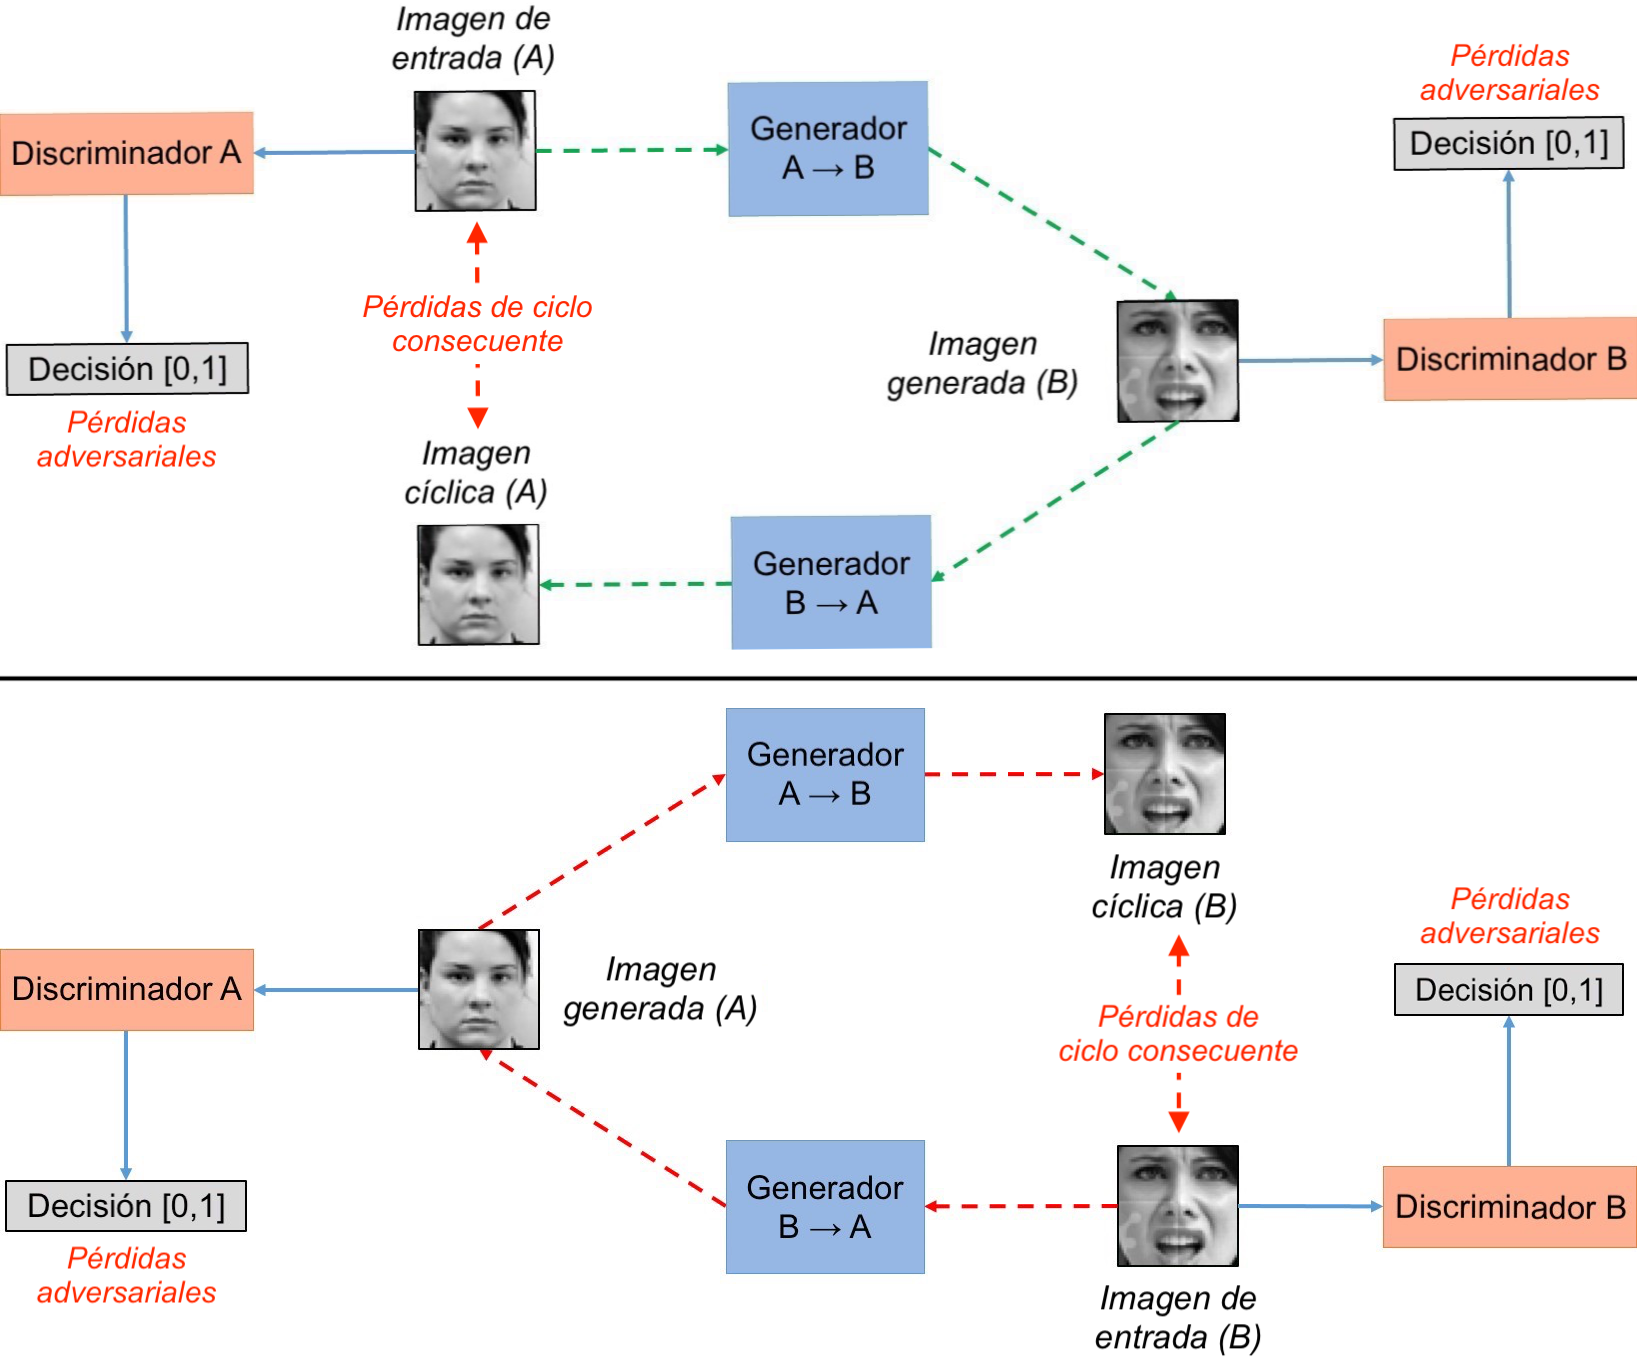
\includegraphics[width=\linewidth]{Images/CycleGANArchitecture.png}
      \caption{Estructura global de la red CycleGAN.}
      \label{fig:CycleGAN_general}
    \end{subfigure}
    
    \vspace{1cm}
    \begin{subfigure}[t]{0.8\textwidth}
      \centering
      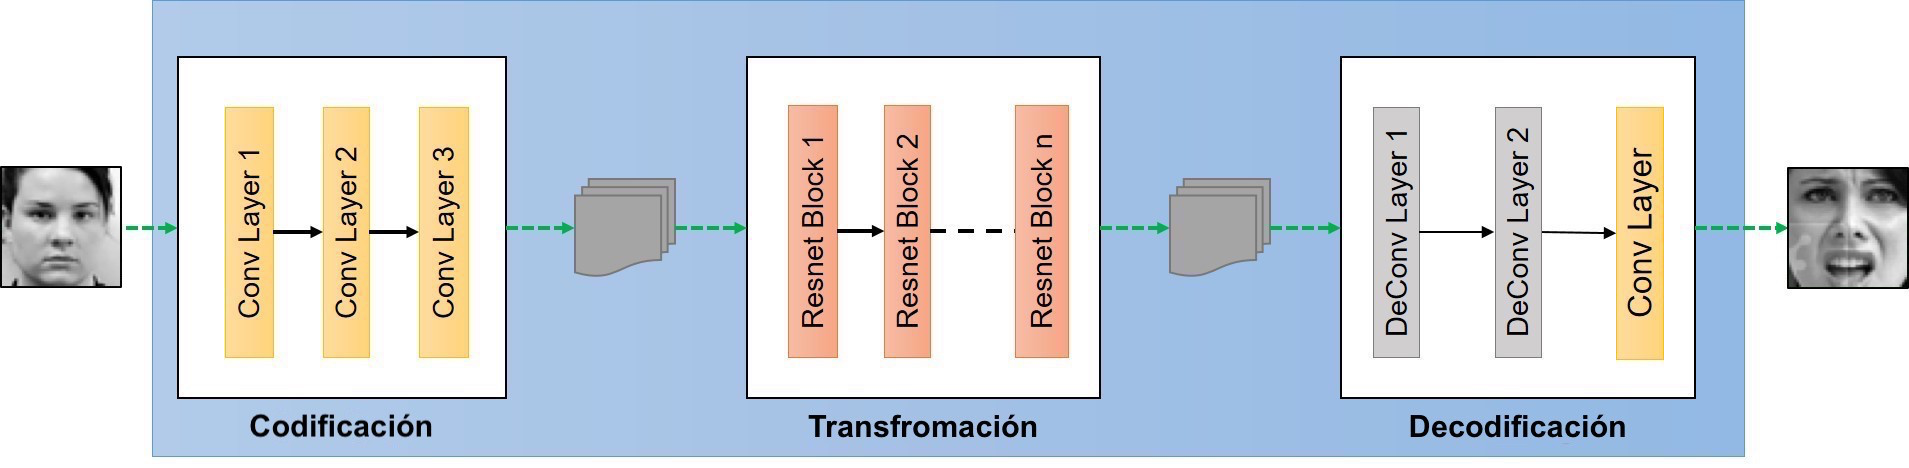
\includegraphics[width=\linewidth]{Images/Generator.png}
      \caption{Arquitectura simplificada del generador de la red CycleGAN.}
      \label{fig:Generator}
    \end{subfigure}
    
    \vspace{1cm}
    \begin{subfigure}[t]{.7\textwidth}
      \centering
      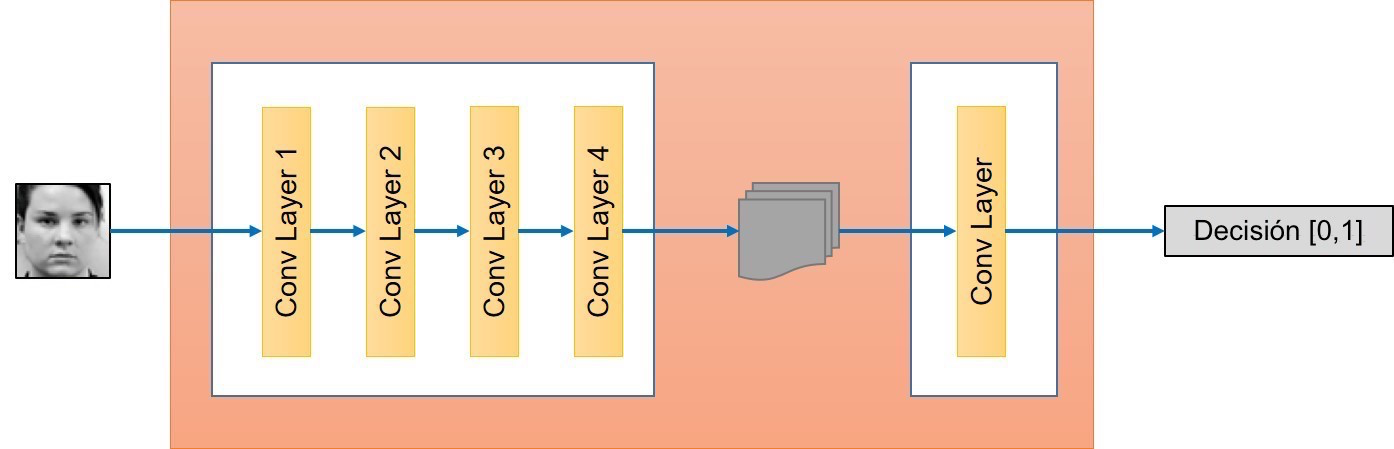
\includegraphics[width=\linewidth]{Images/Discriminator.png}
      \caption{Arquitectura simplificada del discriminador de la red CycleGAN.}
      \label{fig:Discriminator}
    \end{subfigure}
    \caption{Arquitectura esquematizada y simplificada de la Red Generativa Antagónica de Ciclo Consecuente \cite{img:CycleGAN}.}
    \label{fig:CycleGANArchitecture}
\end{figure}

La arquitectura aquí desarrollada y esquematizada en la \autoref{fig:CycleGANArchitecture} es una adaptación de la estructura propuesta en el documento original de las redes CycleGAN y que ha demostrado unos resultados más que razonables en el área de las redes generativas de base neuronal. Asimismo, al igual que los modelos descritos anteriormente, el acondicionamiento se ha llevada a cabo íntegramente en la API de Keras y sobre TensorFlow.

\subsection{Red generadora}

Desde un enfoque de alto nivel es posible dividir la red del generador en 3 módulos distintos dispuestos según la \autoref{fig:Generator}:
\begin{itemize}
    \item \textbf{Módulo de codificación}. Está formado por 3 capas convolucionales que extraen las características superficiales y disminuyen el mapa de activación de la imagen inyectada.
    \item \textbf{Módulo de transformación}. Dado que el objetivo de los procesos de aumento de datos es la retención de ciertas características de la entrada original, como el tamaño y la forma del rostro en este caso, se hace evidente que para este tipo de transformaciones puede resultar especialmente efectivo utilizar arquitecturas residuales, que además favorecen la estabilización de las respuestas de las redes profundas. Es por todo ello que en el contexto particular y en el documento original son empleados básicamente 6 módulos residuales (\autoref{fig:ResNetBlock}) constituidos por filtros convolucionales de tamaño reducido ($3\times 3$).
    \item \textbf{Módulo de decodificación}. Su función es exactamente la opuesta al primer módulo ya que es precisamente el que trata de reconstruir y trasladar la imagen original etiquetada con la emoción neutral al dominio objetivo que corresponde a la expresión de asco. Para tal fin se emplean dos capas deconvolucionales que recomponen el ancho y el alto de la imagen y una última capa convolucional que restaura los canales RGB de la representación inicial.
\end{itemize}

Asimismo, cabe destacar que son utilizadas en cada una de las capas la función de activación ReLU con fugas y la normalización de instancias. Esta última es una sustitución de la técnica de normalización por lotes y es empleada en este proyecto por las mejoras drásticas y demostrables que permite obtener a las redes neuronales profundas en las tareas de generación de datos \cite{InstanceNormalization}. Intuitivamente, este tipo de normalización consigue que la distribución de cada una de las imágenes de un determinado lote parezca gaussiana, lo que permite eliminar información específica y por lo tanto simplificar y optimizar la generación.

En cuanto a la ReLU con fugas, ésta ha reportado mejores resultados en las redes generativas que la ReLU tradicional ya que parece cubrir el espacio de color de una forma más optimizada \cite{GAN}. Igualmente, esta función de activación es el intento de resolver el problema de la muerta de las ReLU convencionales, que para valores menores que cero desactivan la neurona, y por lo tanto del desvanecimiento del gradiente en esas unidades que paralizan el aprendizaje. Su expresión matemática se expone en la \autoref{eq:LeakyReLU}.
\begin{align} \label{eq:LeakyReLU}
    f(x) &= max(x, \alpha x) &\forall \alpha \leq 1 \\
    \text{donde}~ 
    \alpha &\equiv \text{constante} \notag
\end{align}
En el documento original y en el caso particular de este proyecto se toma $\alpha = 0.2$.

\subsection{Red discriminativa}

La función de esta red es básicamente tratar de predecir si la imagen introducida en su entrada es real o procede de la salida del generador. En este caso su arquitectura, representada en la \autoref{fig:Discriminator}, presenta una estructura simple de 5 capas convolucionales de tamaño $4\times 4$ apiladas con una mínima alteración en el último nivel para permitir el cálculo del error de mínimos cuadrados del discriminador \cite{LSGAN}, necesario para realizar la actualización periódica de la función de pérdidas según lo especificado en la \autoref{eq:GAN}. Esta ligera modificación consiste en la supresión de la función de activación y de la unidad de normalización de instancias.

\section{Entrenamiento}

\subsection{Preprocesamiento de los datos}

Teniendo en cuenta la diversidad de las imágenes del conjunto FER-2013, en esta ocasión tan sólo se va a proceder a realizar un preprocesamiento sutil, que además permitirá disminuir el coste computacional de la red. Por ello, se realizan únicamente las siguientes transformaciones:
\begin{itemize}
    \item \textbf{Redimensionamiento}. Dado que la entrada de la arquitectura CycleGAN ha sido ajustada para aceptar las imágenes de la base de datos FER-2013 con la resolución por defecto ($48 \times 48$), tan sólo se realiza una replicación de los datos en escala de gris a los tres espacios de color RGB.
    \item \textbf{Normalización}. El modelo de color RGB de las imágenes de la entrada se adapta al intervalo $[-1, 1]$ mediante la \autoref{eq:PreprocessInception} ya vista anteriormente.
    \item \textbf{Volteo horizontal}. Esta transformación geométrica de carácter aleatorio es la única que se va a aplicar en vista de su eficacia computacional y de enriquecimiento del conjunto de entrada.
\end{itemize}

\subsection{Despliegue en la plataforma Google Cloud}

El proceso de entrenamiento de esta arquitectura ha seguido los puntos descritos en la \autoref{Chapter:CycleGan} y ha tenido como objetivo la reducción de las funciones de pérdidas descritas en la \autoref{eq:CycleGAN} y mostradas gráficamente en la \autoref{fig:CycleGAN_general}. Asimismo, cabe destacar que los parámetros de este modelo han sido escogidos con respecto al artículo original que describe este tipo de redes generativas \cite{cycleGAN}:
\begin{itemize}
    \item \textbf{Inicialización}. En primer lugar y dado que esta red ha sido entrenada desde cero se ha visto necesario realizar una inicialización de los pesos a partir de una distribución gaussiana con una media de $0$ y una desviación estándar de $0.02$. 
    \item \textbf{Tamaño de los lotes}. Las imágenes se han alimentado en la red de una en una, lo que ha implicado también actualizar las funciones de pérdidas y los pesos en cada pasada.
    \item \textbf{Optimizador}. Se ha empleado el optimizador Adam con una tasa de aprendizaje de $ \lambda = 0.0002$ (\autoref{eq:Adam}), $\beta_1 = 0.5$ (\autoref{eq:AdamBeta1}) y $\beta_2 = 0.999$ (\autoref{eq:AdamBeta2}).
    \item \textbf{Peso de la función de pérdidas de ciclo consecuente}. Se le ha otrogado un valor de $\lambda = 10$ (\autoref{eq:CycleGAN}).
    \item \textbf{Iteraciones}. La red ha sido entrenada durante $7\,300$ iteraciones sobre los datos categorizados con las expresiones faciales de asco y neutral.
\end{itemize}

En esta ocasión el entrenamiento en la plataforma de Google Cloud se ha realizado mediante la herramienta Cloud Machine Learning Engine descrita en la \autoref{Chapter:GoogleCloud} y empleando la GPU NVIDIA Tesla K80. Esto es debido a que ya no se presentan las limitaciones de memoria anteriormente existentes al utilizarse esta vez un número bastante inferior de imágenes que reúnen solo las emociones de la clases neutral y asco.

\section{Resultados}